\section{Demo minh họa và thực nghiệm}

\subsection{Mục tiêu thực nghiệm}

    Phần thực nghiệm được xây dựng nhằm kiểm chứng khả năng chạy lại phương pháp CAFE trong bài báo \textit{Generalizable Facial Expression Recognition}, đồng thời đánh giá mức độ tổng quát hóa của mô hình khi huấn luyện trên một miền dữ liệu nguồn và suy luận trực tiếp trên các miền dữ liệu chưa từng được dùng trong huấn luyện. Cụ thể, nhóm đặt ra ba mục tiêu chính.

    Thứ nhất, nhóm tái hiện quy trình huấn luyện CAFE trên RAF-DB, sử dụng mã nguồn chính thức đã được điều chỉnh tối thiểu để phù hợp với môi trường chạy Kaggle. Kết quả huấn luyện được lưu dưới dạng checkpoint \texttt{ours\_best.pth}, \texttt{ours\_final.pth} và nhật ký độ chính xác theo từng epoch.

    Thứ hai, nhóm xây dựng demo suy luận cho bài toán nhận dạng cảm xúc khuôn mặt tĩnh. Demo nhận đầu vào là ảnh khuôn mặt hoặc một thư mục ảnh có nhãn, sau đó trả về nhãn dự đoán thuộc bảy lớp cảm xúc: \textit{surprise}, \textit{fear}, \textit{disgust}, \textit{happy}, \textit{sadness}, \textit{anger} và \textit{neutral}. Ngoài nhãn dự đoán, hệ thống còn xuất điểm tin cậy, file dự đoán chi tiết và ma trận nhầm lẫn để phục vụ phân tích.

    Thứ ba, nhóm mở rộng đánh giá chéo miền trên nhiều bộ dữ liệu khác nhau, bao gồm FERPlus, AffectNet, SFEW2.0, MMAFEDB và CK+48. Các bộ dữ liệu này có điều kiện thu thập, độ phân giải, phân phối lớp và quy ước nhãn khác nhau, do đó phù hợp để kiểm tra giả thuyết cốt lõi của CAFE: mô hình không chỉ cần đạt độ chính xác cao trên tập kiểm thử cùng miền, mà còn phải duy trì hiệu quả khi gặp dữ liệu ngoài miền.


\subsection{Phân tích kỹ thuật từ mã nguồn}

Mã nguồn của repository \texttt{Generalizable-FER} hiện thực ý tưởng chính của phương pháp CAFE theo hướng kết hợp đặc trưng tổng quát của CLIP với một cơ chế chọn lọc đặc trưng theo biểu cảm. Thay vì huấn luyện toàn bộ bộ trích xuất đặc trưng từ đầu trên một tập FER cụ thể, mô hình giữ cố định CLIP ViT-B/32 để lấy biểu diễn ảnh có tính khái quát, sau đó dùng ResNet-18 để sinh mask theo từng ảnh đầu vào. Mask này được đưa qua sigmoid và nhân với feature của CLIP nhằm giữ lại các kênh liên quan đến biểu cảm khuôn mặt, đồng thời giảm ảnh hưởng của các thông tin dễ gây lệch miền như danh tính, nền ảnh, pose hoặc chất lượng ảnh.

\paragraph{Cấu trúc mã nguồn và các tập tin quan trọng.}\mbox{}\\
Phần hiện thực cốt lõi nằm trong file \texttt{code/ours\_CAFE.py}. File này bao gồm định nghĩa dataset \texttt{RafDataset}, kiến trúc ResNet-18 dùng làm mask generator, lớp \texttt{Model}, các hàm phụ cho channel separation và channel dropping, cùng vòng lặp huấn luyện và đánh giá. Thư mục \texttt{code/clip/} chứa phần cài đặt CLIP được gọi bởi \texttt{clip.load("ViT-B/32")}. Ngoài ra, các notebook trong \texttt{code/evaluation\_results\_demo\_trained\_on\_FERPlus/} phục vụ minh họa đánh giá, còn các hình trong \texttt{assets/} hỗ trợ mô tả framework và kết quả.

\paragraph{Luồng xử lý chính của mô hình.}\mbox{}\\
Trong \texttt{Model.forward()}, ảnh đầu vào \texttt{x} được đưa qua hai nhánh song song. Nhánh thứ nhất dùng CLIP để trích xuất feature ảnh:
\begin{lstlisting}[language=Python]
with torch.no_grad():
    image_features = clip_model.encode_image(x)
\end{lstlisting}
Việc đặt \texttt{encode\_image()} trong \texttt{torch.no\_grad()} cho thấy CLIP không được cập nhật trọng số trong quá trình train. Đây là lựa chọn quan trọng đối với bài toán generalizable FER, vì CLIP đã được pretrain trên dữ liệu lớn và có biểu diễn tổng quát hơn so với một backbone chỉ học trên dataset nguồn như RAF-DB.

Nhánh thứ hai dùng ResNet-18 để tạo vector 512 chiều từ cùng ảnh đầu vào. Vector này không được dùng trực tiếp làm logits phân loại, mà đóng vai trò mask thô. Vì CLIP ViT-B/32 cũng trả về feature 512 chiều, hai vector có thể được nhân từng kênh:
\begin{lstlisting}[language=Python]
x = image_features * torch.sigmoid(x)
out = self.fc(x)
\end{lstlisting}
Cơ chế này có thể tóm tắt bằng công thức:
\[
F = \mathrm{CLIP}(x), \quad
M = \mathrm{ResNet18}(x), \quad
\widetilde{F} = F \odot \sigma(M), \quad
\hat{y} = \mathrm{FC}(\widetilde{F}).
\]
Trong đó, \(F\) là feature tổng quát từ CLIP, \(M\) là mask do ResNet-18 sinh ra, \(\sigma(M)\) là mask mềm trong khoảng \([0,1]\), \(\widetilde{F}\) là feature đã được chọn lọc theo biểu cảm, và \(\hat{y}\) là logits của 7 lớp cảm xúc.

\paragraph{Vai trò của sigmoid mask.}\mbox{}\\
Sigmoid là thành phần then chốt vì nó biến output của ResNet-18 thành một bộ lọc mềm theo kênh. Giá trị gần 1 nghĩa là kênh CLIP tương ứng được giữ lại nhiều, còn giá trị gần 0 nghĩa là kênh đó bị giảm ảnh hưởng. Nhờ giới hạn mask trong khoảng \([0,1]\), mô hình không đảo dấu hoặc khuếch đại tùy ý feature CLIP. Nếu bỏ sigmoid và nhân trực tiếp với output ResNet, mask có thể nhận giá trị âm hoặc quá lớn, làm biến dạng biểu diễn tổng quát của CLIP và tăng nguy cơ overfit vào miền dữ liệu nguồn.

\paragraph{Classifier và các hàm mất mát phụ.}\mbox{}\\
Sau khi có masked feature, source dùng một fully connected layer \texttt{nn.Linear(512, 7)} để dự đoán 7 lớp biểu cảm. Loss chính là cross entropy giữa output này và nhãn thật. Bên cạnh đó, trong pha train, hàm \texttt{supervisor()} tạo thêm hai loss phụ: channel separation loss và channel-diverse loss. Source gom feature 512 chiều thành các nhóm kênh, dùng \texttt{my\_MaxPool2d(..., cnum=73)} để lấy phản hồi mạnh nhất theo nhóm, rồi tính cross entropy phụ với nhãn. Cơ chế này ép feature sau mask không chỉ đúng qua FC classifier, mà còn có cấu trúc phân biệt theo từng nhóm cảm xúc.

Channel dropping được hiện thực trong hàm \texttt{Mask(nb\_batch)}. Hàm này tạo mask nhị phân để random drop một số kênh trong từng nhóm khi train. Mục tiêu là tránh việc mô hình phụ thuộc vào một vài kênh mạnh cố định; thay vào đó, thông tin biểu cảm phải được phân bố ổn định hơn trên nhiều kênh. Tổng loss trong vòng lặp train được tính như sau:
\begin{lstlisting}[language=Python]
loss1 = nn.CrossEntropyLoss()(output, labels)
loss = loss1 + 5 * MC_loss[1] + 1.5 * MC_loss[0]
\end{lstlisting}
Trong đó, \texttt{loss1} là classification loss chính, \texttt{MC\_loss[0]} là channel separation loss, còn \texttt{MC\_loss[1]} là channel-diverse loss. Hai hệ số 1.5 và 5 đóng vai trò cân bằng giữa mục tiêu phân loại và các ràng buộc regularization trên feature.

\paragraph{Tiền xử lý dữ liệu và quy trình huấn luyện.}\mbox{}\\
\texttt{RafDataset} đọc nhãn từ thư mục \texttt{EmoLabel}, lấy ảnh đã căn chỉnh từ \texttt{Image/aligned}, sau đó đưa label về miền \([0,6]\) tương ứng với 7 lớp cảm xúc. Trong huấn luyện, ảnh được resize về \(224 \times 224\), chuyển sang tensor, normalize theo mean/std ImageNet, đồng thời có augmentation như horizontal flip, Gaussian noise và random erasing. Khi đánh giá, source vẫn resize và normalize nhưng bỏ các augmentation ngẫu nhiên. Quy trình train dùng Adam với learning rate \(2 \times 10^{-4}\), weight decay \(10^{-4}\), scheduler ExponentialLR và lưu checkpoint \texttt{ours\_best.pth} khi accuracy tốt hơn.

\paragraph{Suy luận và khác biệt giữa train/test.}\mbox{}\\
Ở pha test, \texttt{Model.forward()} không gọi \texttt{supervisor()} và không dùng channel dropping. Mô hình chỉ tính feature CLIP, sinh sigmoid mask bằng ResNet-18, nhân hai feature lại với nhau, rồi đưa qua FC classifier để lấy dự đoán cuối cùng. Điều này hợp lý vì channel separation, channel dropping và channel-diverse loss chỉ có nhiệm vụ định hướng quá trình học representation; khi suy luận, việc giữ các yếu tố ngẫu nhiên như dropping có thể làm output kém ổn định.

\paragraph{Tác động nếu thay đổi hoặc loại bỏ thành phần quan trọng.}\mbox{}\\
Nếu bỏ CLIP cố định, mô hình mất nền tảng feature tổng quát và dễ trở thành một FER backbone thông thường, có nguy cơ học các đặc trưng riêng của dataset nguồn. Nếu fine-tune CLIP trực tiếp, accuracy trên source domain có thể tăng nhưng khả năng tổng quát sang dataset khác có thể giảm do domain overfitting. Nếu bỏ ResNet-18 mask generator hoặc phép nhân \texttt{image\_features * torch.sigmoid(x)}, mô hình gần như chỉ còn CLIP cộng classifier, không còn cơ chế chọn lọc kênh theo từng ảnh đầu vào. Nếu bỏ các loss phụ trong \texttt{supervisor()}, mô hình vẫn train được bằng cross entropy chính, nhưng feature sau mask thiếu ràng buộc class-wise và có thể phụ thuộc nhiều hơn vào FC classifier.

Nhìn chung, điểm cốt lõi của source code không chỉ là ``dùng CLIP'', mà là dùng CLIP ở trạng thái cố định và học một sigmoid mask để chọn ra phần feature liên quan đến biểu cảm. ResNet-18 đảm nhiệm việc sinh mask thích ứng theo ảnh, FC classifier tạo output cuối cùng, còn channel separation, channel dropping và channel-diverse loss đóng vai trò regularization giúp feature có cấu trúc hơn. Sự kết hợp này giải thích vì sao CAFE hướng tới mục tiêu tổng quát hóa tốt hơn so với cách huấn luyện end-to-end truyền thống trên một tập FER đơn lẻ.


\subsection{Thiết lập thực nghiệm}
% \begin{table}[H]
%     \centering
%     \caption{Thiết lập thực nghiệm}
%     \begin{tabularx}{\textwidth}{L{4cm} X}
%         \toprule
%         \textbf{Thành phần} & \textbf{Mô tả} \\
%         \midrule
%         Bộ dữ liệu & \textit{[Điền tên dataset, số lượng mẫu, cách chia train/validation/test]} \\
%         Phần cứng & \textit{[CPU/GPU/RAM hoặc môi trường chạy]} \\
%         Phần mềm & \textit{[Hệ điều hành, Python, framework, phiên bản thư viện]} \\
%         Siêu tham số & \textit{[Batch size, learning rate, epoch, optimizer, ngưỡng quyết định]} \\
%         Giao thức đánh giá & \textit{[Cách đo Accuracy, EER, mAP, Rank-1, v.v.]} \\
%         \bottomrule
%     \end{tabularx}
% \end{table}

Bảng \ref{tab:demo_setup} tóm tắt cấu hình thực nghiệm chính. RAF-DB được dùng làm bộ dữ liệu nguồn để huấn luyện. Sau đó, checkpoint tốt nhất được đánh giá trực tiếp trên các bộ dữ liệu khác mà không tinh chỉnh lại, đúng với tinh thần đánh giá zero-shot cross-dataset của bài báo.

\begin{table}[htbp]
\centering
\caption{Thiết lập thực nghiệm}
\label{tab:demo_setup}
\begin{tabular}{p{0.22\linewidth}p{0.68\linewidth}}
\hline
\textbf{Thành phần} & \textbf{Mô tả} \\
\hline
Bộ dữ liệu huấn luyện & RAF-DB, sử dụng bảy lớp cảm xúc theo thứ tự: surprise, fear, disgust, happy, sadness, anger, neutral. \\
Bộ dữ liệu đánh giá & RAF-DB test, FERPlus test, AffectNet Test, SFEW2.0 Val, MMAFEDB test và CK+48. Các lớp contempt bị loại bỏ vì mô hình không có đầu ra tương ứng. \\
Phần cứng & Kaggle Notebook có GPU, sử dụng thiết bị \texttt{cuda:0} trong quá trình huấn luyện và đánh giá. \\
Phần mềm & Python, PyTorch, torchvision, OpenCV, PIL, NumPy, pandas, scikit-learn, matplotlib, seaborn và CLIP ViT-B/32. \\
Tiền xử lý & Chuyển ảnh sang RGB, resize về $224 \times 224$, chuẩn hóa theo ImageNet. Với CK+48, ảnh 48 $\times$ 48 được phóng lên $224 \times 224$. \\
Siêu tham số huấn luyện & 60 epoch, batch size 32, Adam, learning rate $0.0002$, weight decay $10^{-4}$, ExponentialLR $\gamma=0.9$, seed 3407. \\
Giao thức đánh giá & Không tinh chỉnh trên miền đích; đo Overall Accuracy, Mean Accuracy, Macro-F1, độ chính xác từng lớp và ma trận nhầm lẫn. \\
\hline
\end{tabular}
\end{table}

Trong số các bộ dữ liệu được sử dụng để đánh giá chéo miền, tập dữ liệu mở rộng CK+48 là một trường hợp đặc biệt được thu thập trong điều kiện phòng thí nghiệm. Khác với các tập dữ liệu tự nhiên (in-the-wild), tiến trình ghi nhận biểu cảm của CK+48 bắt đầu từ trạng thái trung tính (\textit{neutral}) cho đến khi biểu cảm đạt đỉnh điểm (\textit{peak}). Để phân tích sâu sắc ảnh hưởng của cấu trúc dữ liệu đối với mô hình GFER, nhóm đã thiết lập đánh giá CK+48 trên hai chế độ riêng biệt:
\begin{enumerate}
    \item \textbf{CK+48 7 lớp (gồm Neutral):} Đánh giá trên toàn bộ tiến trình biểu cảm bao gồm cả trạng thái trung tính. Như thể hiện ở Hình~\ref{fig:ck_dist_7}, chế độ này có sự mất cân bằng dữ liệu cực kỳ lớn với lớp trung tính chiếm ưu thế tuyệt đối (593 trên tổng số 902 mẫu), trong khi các lớp khó như sợ hãi (\textit{fear}) chỉ có 25 mẫu.
    \item \textbf{CK+48 6 lớp peak-only:} Loại bỏ hoàn toàn lớp trung tính và chỉ đánh giá trên các mẫu ảnh biểu cảm đạt đỉnh. Chế độ này (Hình~\ref{fig:ck_dist_6}) giúp phân phối giữa các cảm xúc cân bằng hơn, nhưng tổng số mẫu kiểm thử giảm mạnh xuống còn 309 mẫu.
\end{enumerate}

\begin{figure}[htbp]
    \centering
    \begin{minipage}{0.48\textwidth}
        \centering
        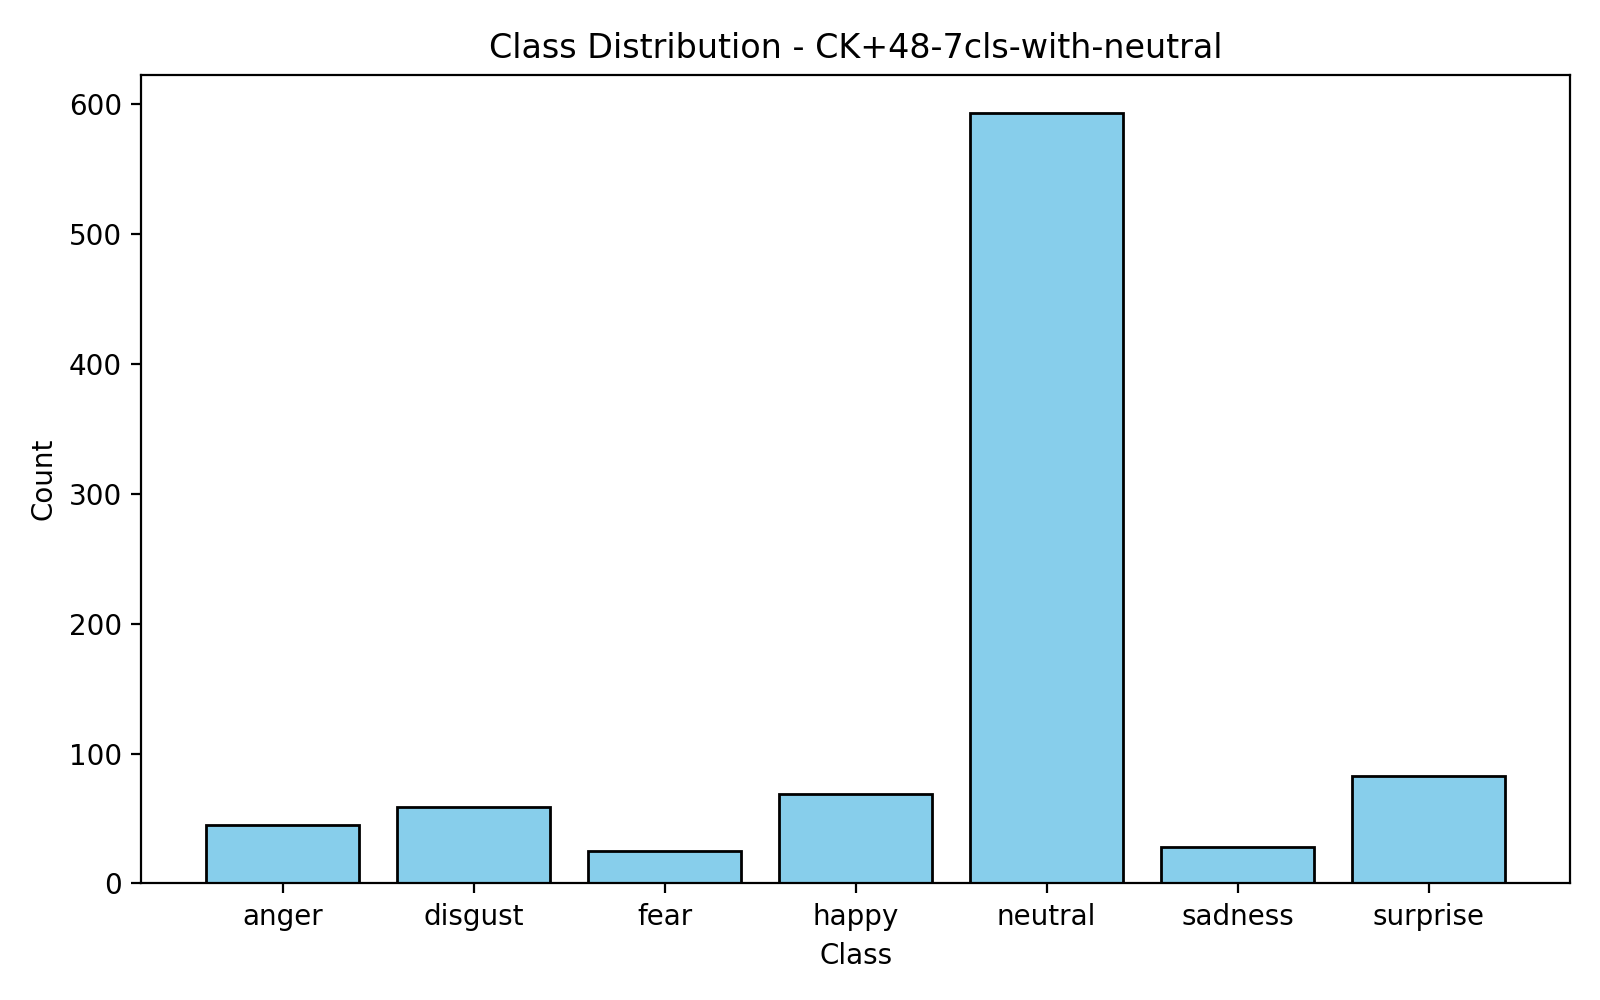
\includegraphics[width=\textwidth]{images/class_distribution_2.png}
        \caption{Phân phối mẫu CK+48 ở chế độ 7 lớp (gồm Neutral).}
        \label{fig:ck_dist_7}
    \end{minipage}
    \hfill
    \begin{minipage}{0.48\textwidth}
        \centering
        
\includegraphics[width=\textwidth]{images/class_distribution.png}
        \caption{Phân phối mẫu CK+48 ở chế độ 6 lớp peak-only.}
        \label{fig:ck_dist_6}
    \end{minipage}
    \caption{So sánh phân phối số lượng mẫu của bộ dữ liệu CK+48 ở hai chế độ đánh giá.}
    \label{fig:ckplus_distribution}
\end{figure}

\subsection{Kết quả thực nghiệm}
% Trình bày kết quả thu được bằng bảng, biểu đồ hoặc hình minh họa. Nếu kết quả không khớp hoàn toàn với bài báo, cần ghi rõ mức sai khác và lý do hợp lý.

% \begin{table}[H]
%     \centering
%     \caption{So sánh kết quả thực nghiệm với bài báo gốc}
%     \begin{tabularx}{\textwidth}{L{3.2cm} C{3cm} C{3cm} X}
%         \toprule
%         \textbf{Chỉ số} & \textbf{Bài báo gốc} & \textbf{Nhóm thực nghiệm} & \textbf{Nhận xét} \\
%         \midrule
%         \textit{[Metric 1]} & \textit{[Giá trị]} & \textit{[Giá trị]} & \textit{[Phân tích]} \\
%         \textit{[Metric 2]} & \textit{[Giá trị]} & \textit{[Giá trị]} & \textit{[Phân tích]} \\
%         \bottomrule
%     \end{tabularx}
% \end{table}


Trên RAF-DB, mô hình đạt độ chính xác tốt nhất 89.15\% tại epoch 41 và lặp lại mức này tại epoch 57. Độ chính xác tăng nhanh trong 10 epoch đầu, từ 69.10\% lên 87.91\%, sau đó hội tụ quanh vùng 88.8--89.1\%. Kết quả này cho thấy quá trình huấn luyện ổn định và checkpoint cuối không bị suy giảm mạnh so với checkpoint tốt nhất; tại epoch 60, độ chính xác đạt 88.92\%.

Bảng \ref{tab:paper_compare} so sánh kết quả của nhóm với các giá trị được báo cáo trong bài báo gốc đối với thiết lập huấn luyện trên RAF-DB. Nhìn chung, kết quả tái hiện trên RAF-DB cao hơn nhẹ so với bài báo gốc. Trên MMAFEDB, kết quả gần như tương đương. Trên AffectNet, kết quả của nhóm cao hơn giá trị tham chiếu. Tuy nhiên, trên FERPlus và SFEW2.0, độ chính xác thấp hơn bài báo, phản ánh ảnh hưởng của khác biệt dữ liệu, cấu trúc thư mục, tiền xử lý và điều kiện chạy lại.

\begin{table}[htbp]
\centering
\caption{So sánh kết quả thực nghiệm với bài báo gốc}
\label{tab:paper_compare}
\begin{tabular}{lccc}
\hline
\textbf{Tập đánh giá} & \textbf{Bài báo gốc OA (\%)} & \textbf{Nhóm thực nghiệm OA (\%)} & \textbf{Sai khác} \\
\hline
RAF-DB & 88.72 & 89.15 & +0.43 \\
FERPlus & 73.16 & 66.81 & -6.35 \\
AffectNet & 45.86 & 52.01 & +6.15 \\
SFEW2.0 & 52.86 & 46.87 & -5.99 \\
MMAFEDB & 56.80 & 56.72 & -0.08 \\
Trung bình & 63.48 & 62.31 & -1.17 \\
\hline
\end{tabular}
\end{table}

Bên cạnh Overall Accuracy, nhóm tính thêm Mean Accuracy và Macro-F1 để đánh giá cân bằng hơn trong bối cảnh dữ liệu mất cân bằng lớp. Bảng \ref{tab:cross_dataset_results} trình bày kết quả chi tiết. FERPlus đạt 66.81\% OA, 56.24\% MA và 53.06\% Macro-F1. AffectNet đạt 52.01\% OA, 46.93\% MA và 43.97\% Macro-F1. MMAFEDB đạt 56.72\% OA, gần sát kết quả bài báo gốc, nhưng MA chỉ đạt 42.95\%, cho thấy mô hình vẫn thiên về các lớp có số lượng mẫu lớn. SFEW2.0 là tập khó nhất trong thí nghiệm, chỉ đạt 46.87\% OA và 33.98\% Macro-F1 do ảnh trong môi trường phim có nhiều biến thiên về ánh sáng, góc mặt và che khuất.

\begin{table}[htbp]
\centering
\caption{Kết quả đánh giá chéo miền và mở rộng}
\label{tab:cross_dataset_results}
\begin{tabular}{lrrrr}
\hline
\textbf{Tập dữ liệu} & \textbf{Số mẫu} & \textbf{OA (\%)} & \textbf{MA (\%)} & \textbf{Macro-F1 (\%)} \\
\hline
CK+48, 6 lớp peak-only & 309 & 64.72 & 52.26 & 51.43 \\
CK+48, 7 lớp có neutral & 902 & 82.48 & 57.90 & 53.73 \\
FERPlus test & 3543 & 66.81 & 56.24 & 53.06 \\
AffectNet Test & 13206 & 52.01 & 46.93 & 43.97 \\
SFEW2.0 Val & 431 & 46.87 & 38.78 & 33.98 \\
MMAFEDB test & 17356 & 56.72 & 42.95 & 43.17 \\
\hline
\end{tabular}
\end{table}

Bảng~\ref{tab:per_class_acc} trình bày độ chính xác theo từng lớp cảm xúc trên tất cả các tập dữ liệu đánh giá. Kết quả cho thấy mô hình nhận dạng tốt nhất các biểu cảm có dấu hiệu hình học rõ ràng: \textit{happy} luôn đạt trên 75\% trên mọi tập, \textit{surprise} và \textit{neutral} cũng đạt mức cao. Ngược lại, \textit{fear} hoàn toàn thất bại với 0\% trên CK+48 (cả hai chế độ) và SFEW2.0, chỉ đạt 4.4\% trên AffectNet và 8.2\% trên MMAFEDB --- đây là lớp yếu nhất xuyên suốt mọi tập. \textit{Disgust} cũng có kết quả thấp đồng đều (4.3\%--28.6\%), phản ánh sự khan hiếm mẫu và độ khó phân biệt cao của hai cảm xúc này.

\begin{table}[htbp]
\centering
\caption{Độ chính xác theo từng lớp cảm xúc (\%) trên các tập đánh giá chéo miền}
\label{tab:per_class_acc}
\setlength{\tabcolsep}{4pt}
\begin{tabular}{lrrrrrrr}
\hline
\textbf{Tập dữ liệu} & \textbf{Surprise} & \textbf{Fear} & \textbf{Disgust} & \textbf{Happy} & \textbf{Sadness} & \textbf{Anger} & \textbf{Neutral} \\
\hline
CK+48 7cls      & 95.18 & 0.00  & 55.93 & 100.00 & 53.57 &  8.89 & 91.74 \\
CK+48 6cls peak & 95.18 & 0.00  & 55.93 & 100.00 & 53.57 &  8.89 & --- \\
FERPlus         & 68.22 & 31.63 & 28.57 &  94.51 & 67.93 & 49.38 & 53.45 \\
AffectNet       & 61.67 &  4.39 & 18.51 &  83.43 & 60.04 & 31.66 & 68.83 \\
SFEW2.0         & 12.50 &  0.00 &  4.35 &  86.11 & 68.49 & 28.57 & 71.43 \\
MMAFEDB         & 56.00 &  8.25 & 17.25 &  75.87 & 45.11 & 42.07 & 56.09 \\
\hline
\end{tabular}
\end{table}

Hình~\ref{fig:cm_all} trình bày ma trận nhầm lẫn trên sáu tập đánh giá, cho phép quan sát trực tiếp các pattern lỗi đặc trưng của mô hình CAFE khi hoạt động trong điều kiện zero-shot cross-domain.

\begin{figure}[htbp]
    \centering
    \begin{minipage}{0.48\textwidth}
        \centering
        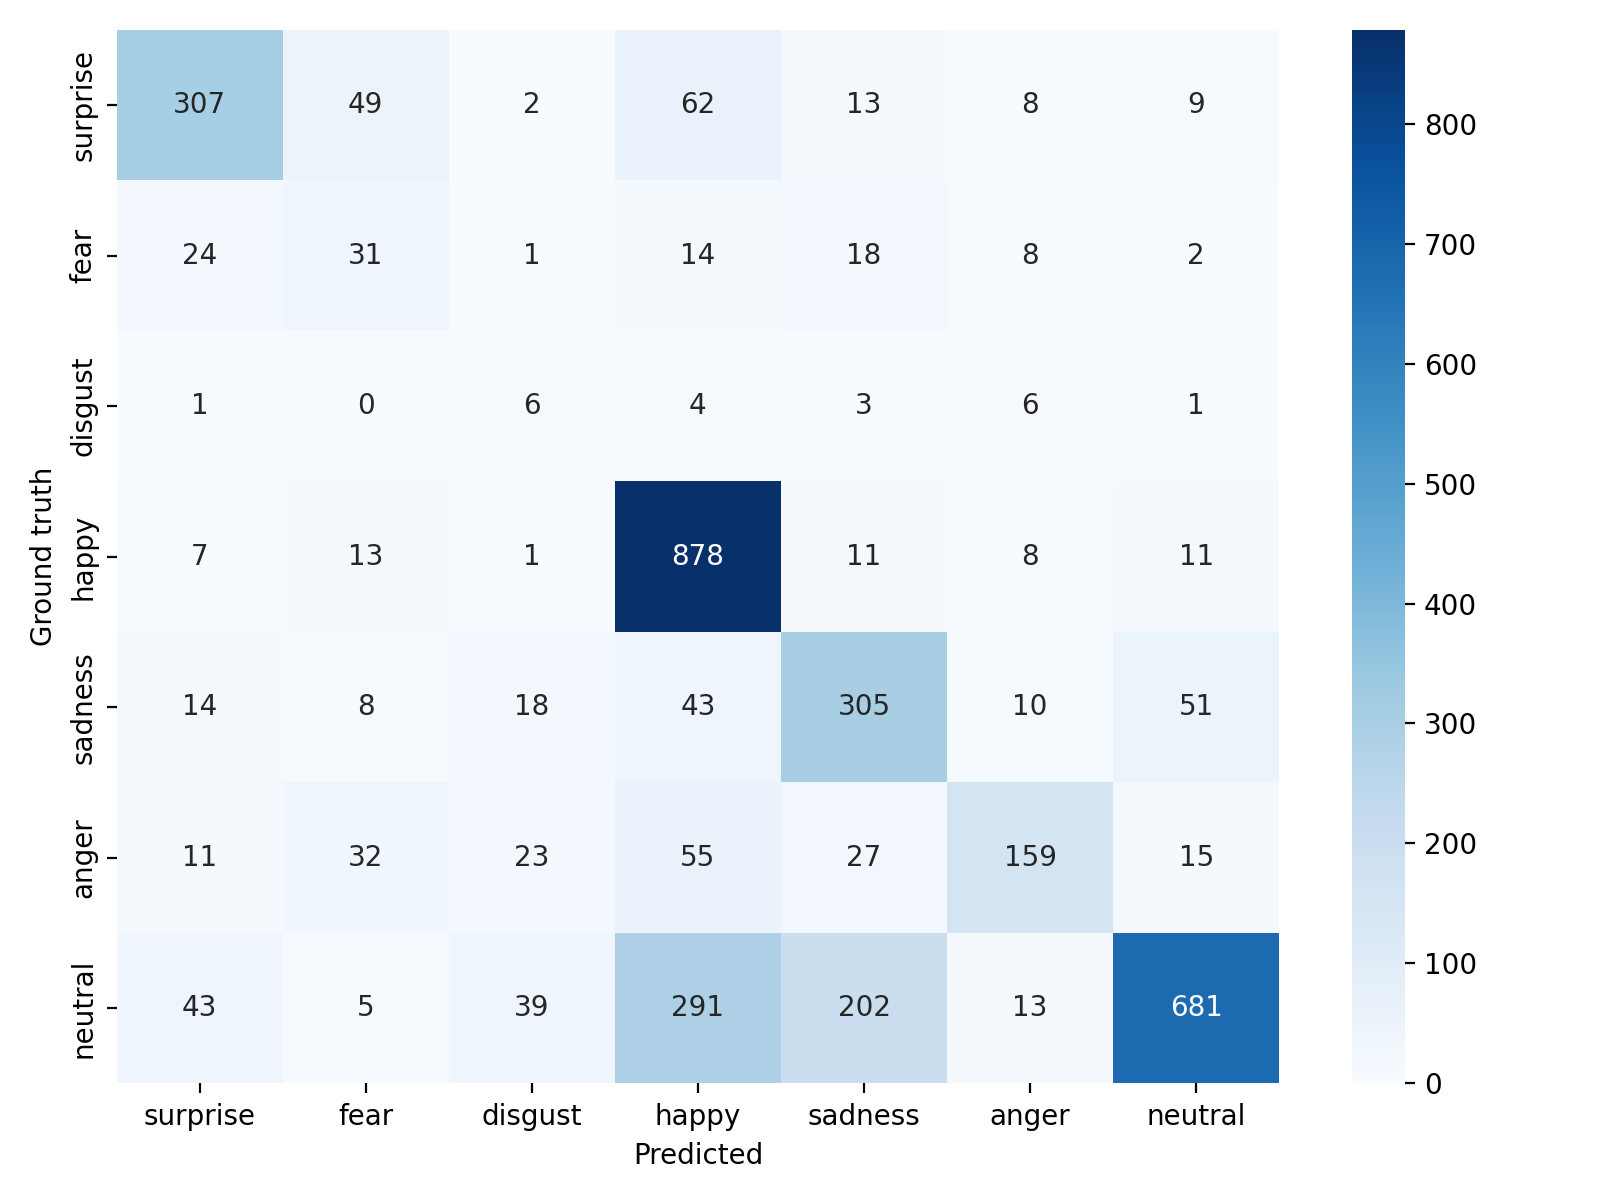
\includegraphics[width=\textwidth]{images/cm_ferplus.png}
        \caption*{(a) FERPlus (3543 mẫu)}
    \end{minipage}
    \hfill
    \begin{minipage}{0.48\textwidth}
        \centering
        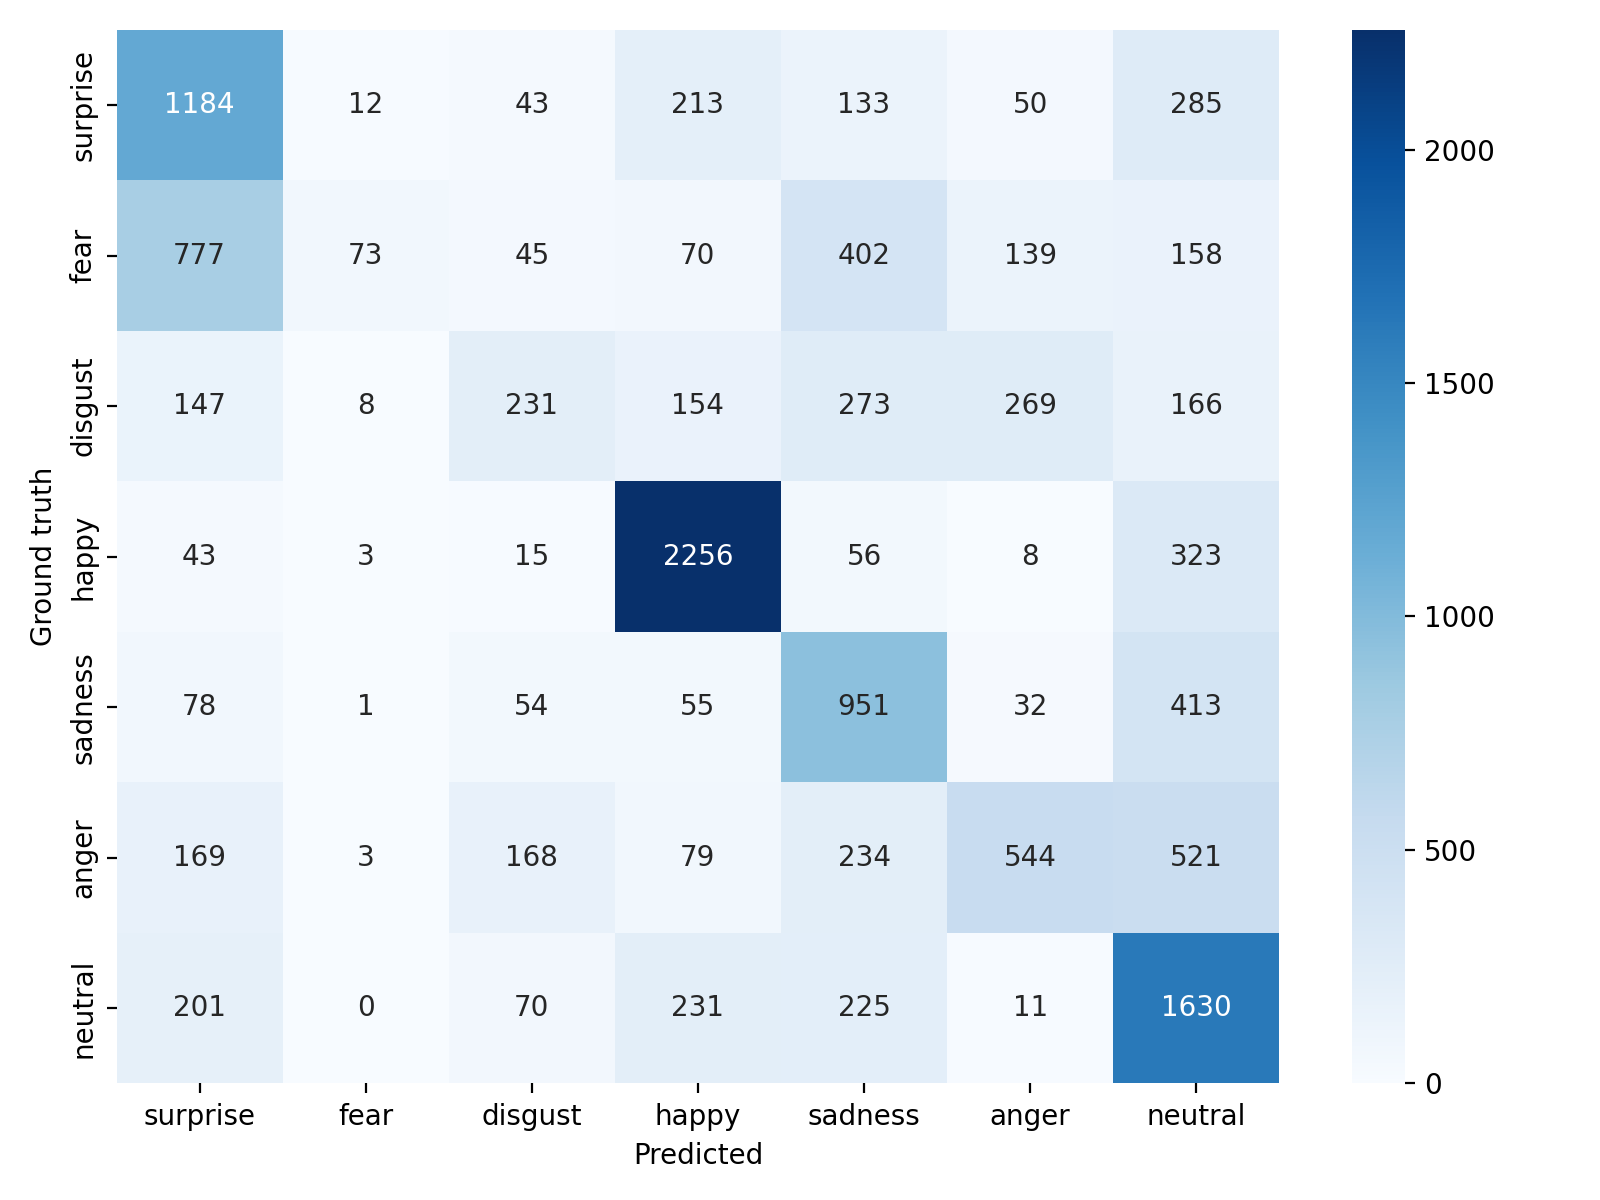
\includegraphics[width=\textwidth]{images/cm_affectnet.png}
        \caption*{(b) AffectNet (13206 mẫu)}
    \end{minipage}

    \vspace{0.5em}

    \begin{minipage}{0.48\textwidth}
        \centering
        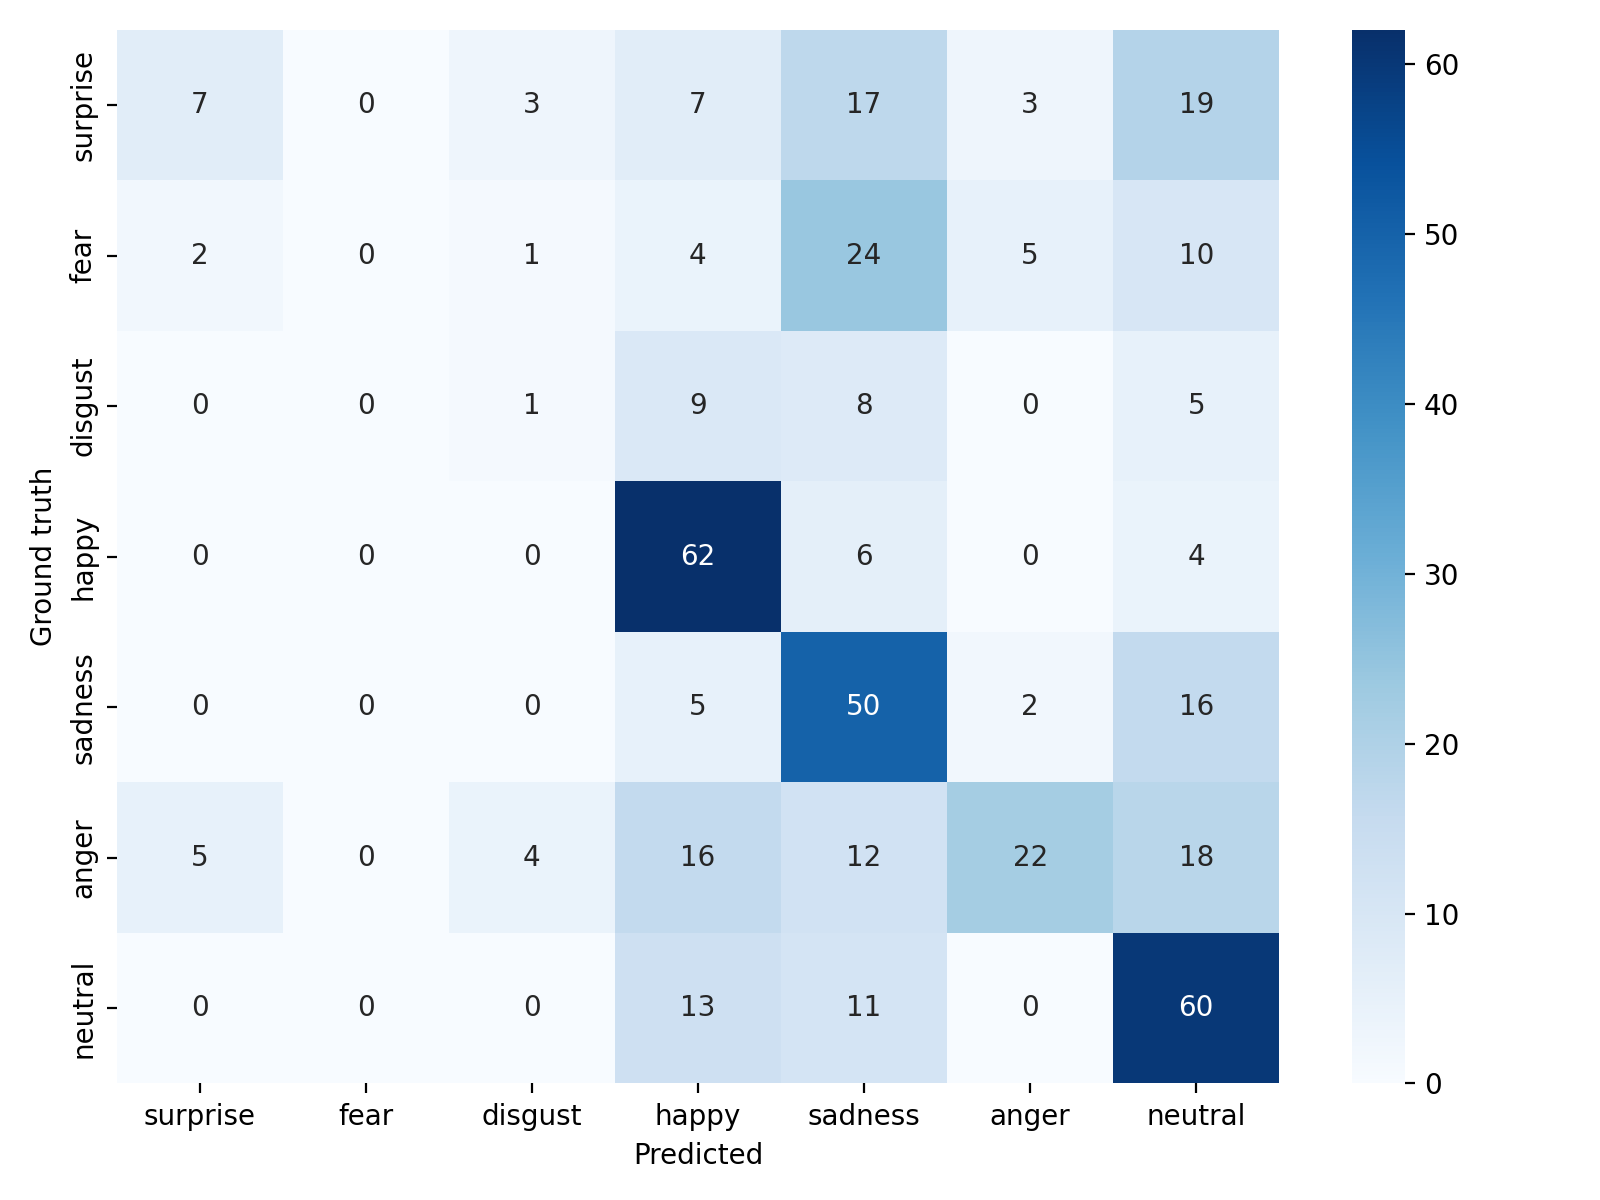
\includegraphics[width=\textwidth]{images/cm_sfew.png}
        \caption*{(c) SFEW2.0 Val (431 mẫu)}
    \end{minipage}
    \hfill
    \begin{minipage}{0.48\textwidth}
        \centering
        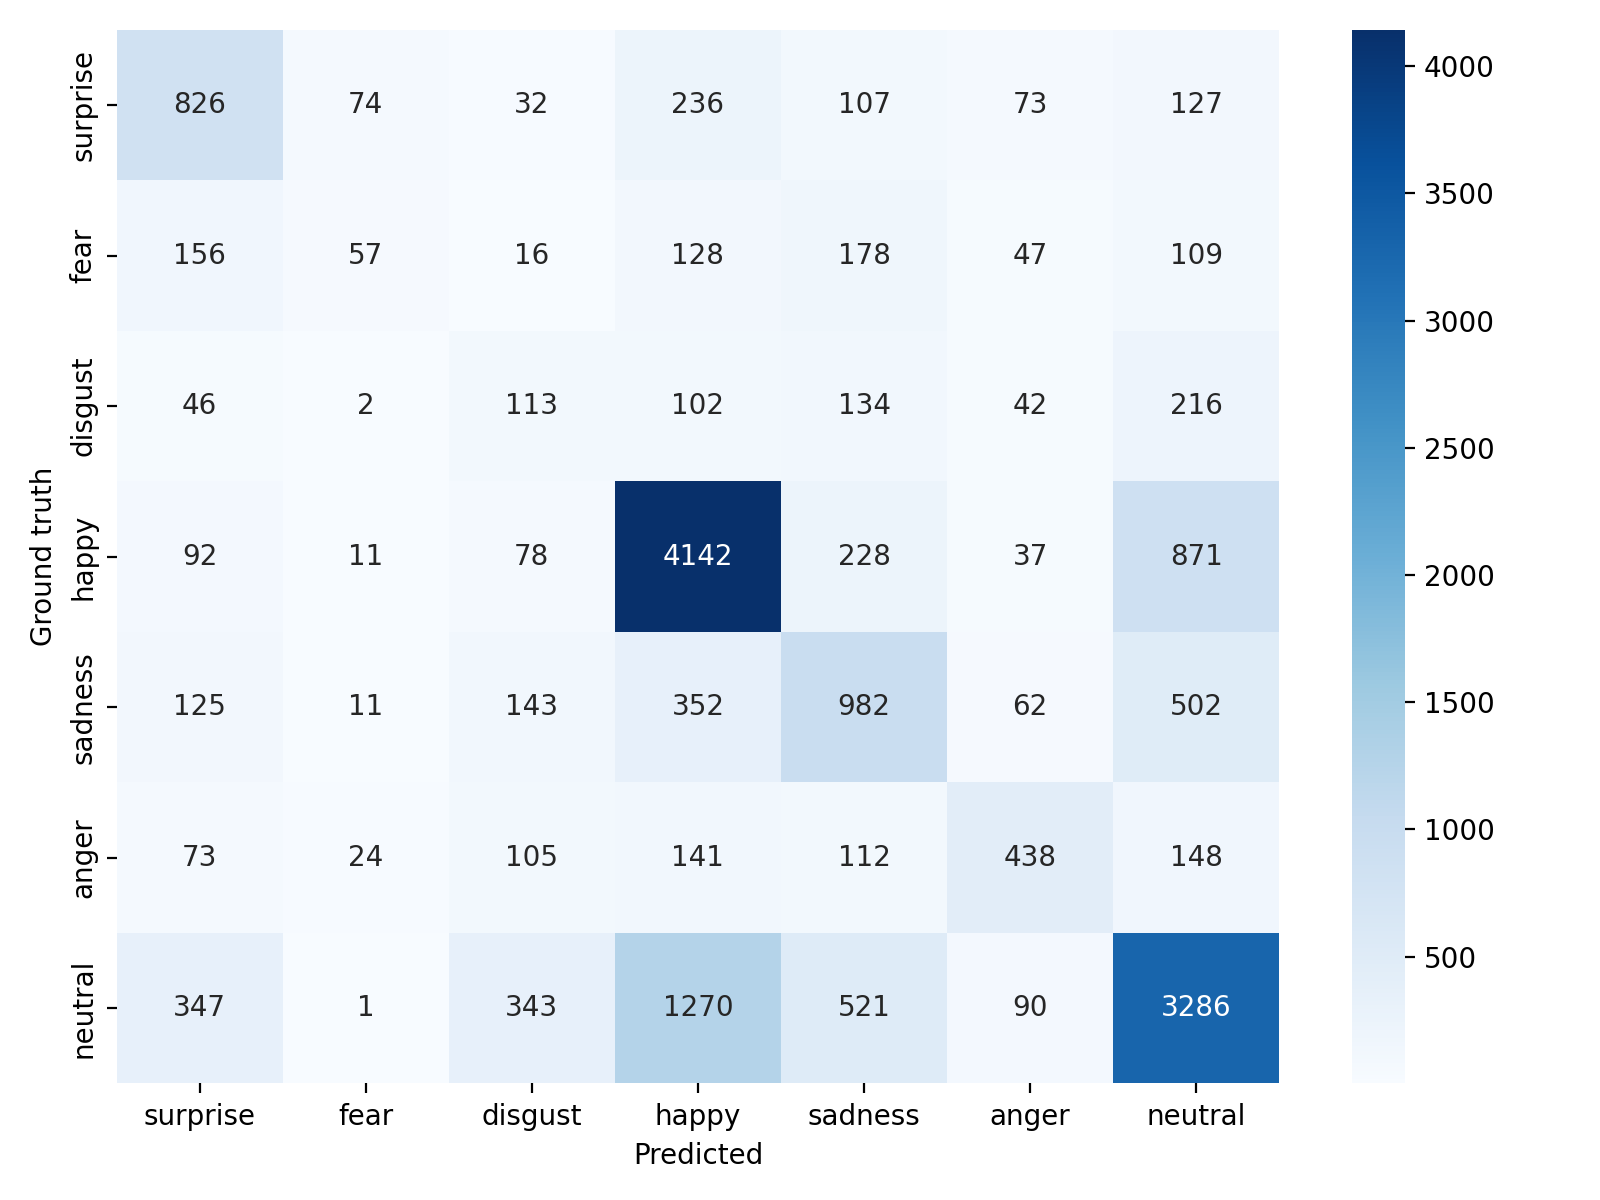
\includegraphics[width=\textwidth]{images/cm_mma.png}
        \caption*{(d) MMAFEDB (17356 mẫu)}
    \end{minipage}

    \vspace{0.5em}

    \begin{minipage}{0.48\textwidth}
        \centering
        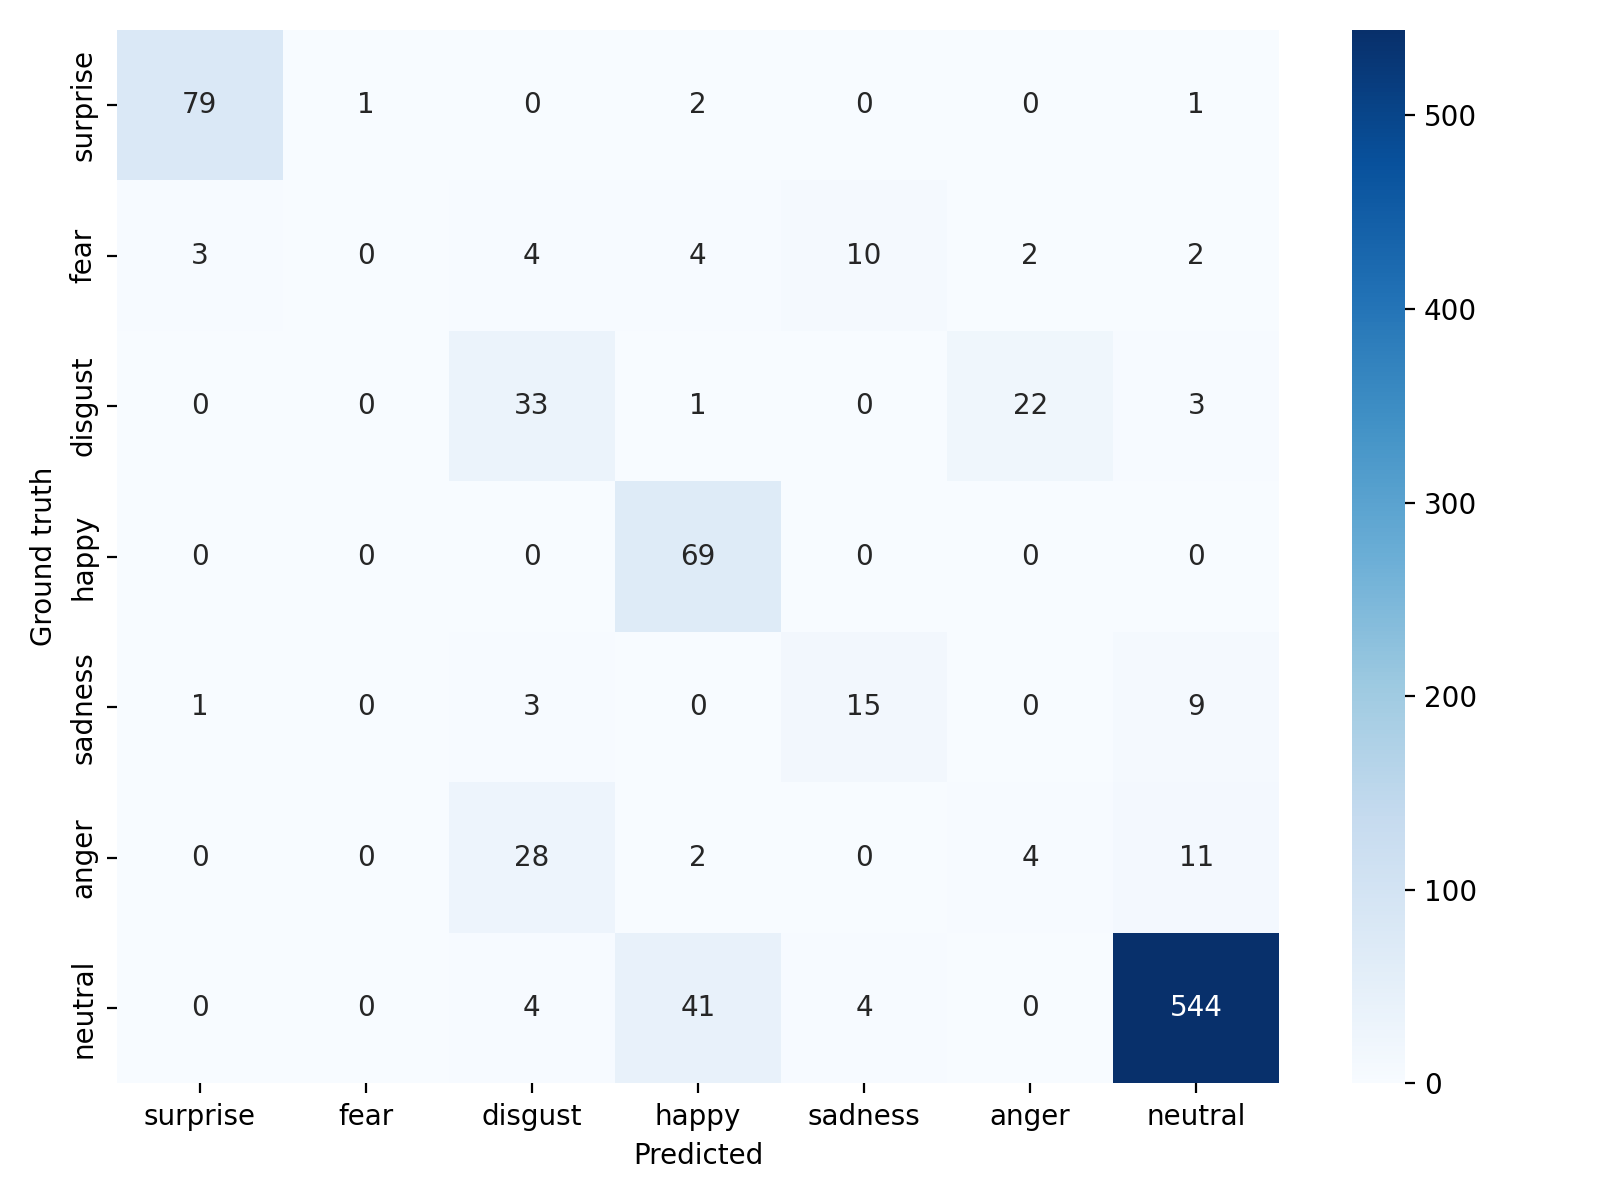
\includegraphics[width=\textwidth]{images/cm_ckplus48_7cls.png}
        \caption*{(e) CK+48 7 lớp có Neutral (902 mẫu)}
    \end{minipage}
    \hfill
    \begin{minipage}{0.48\textwidth}
        \centering
        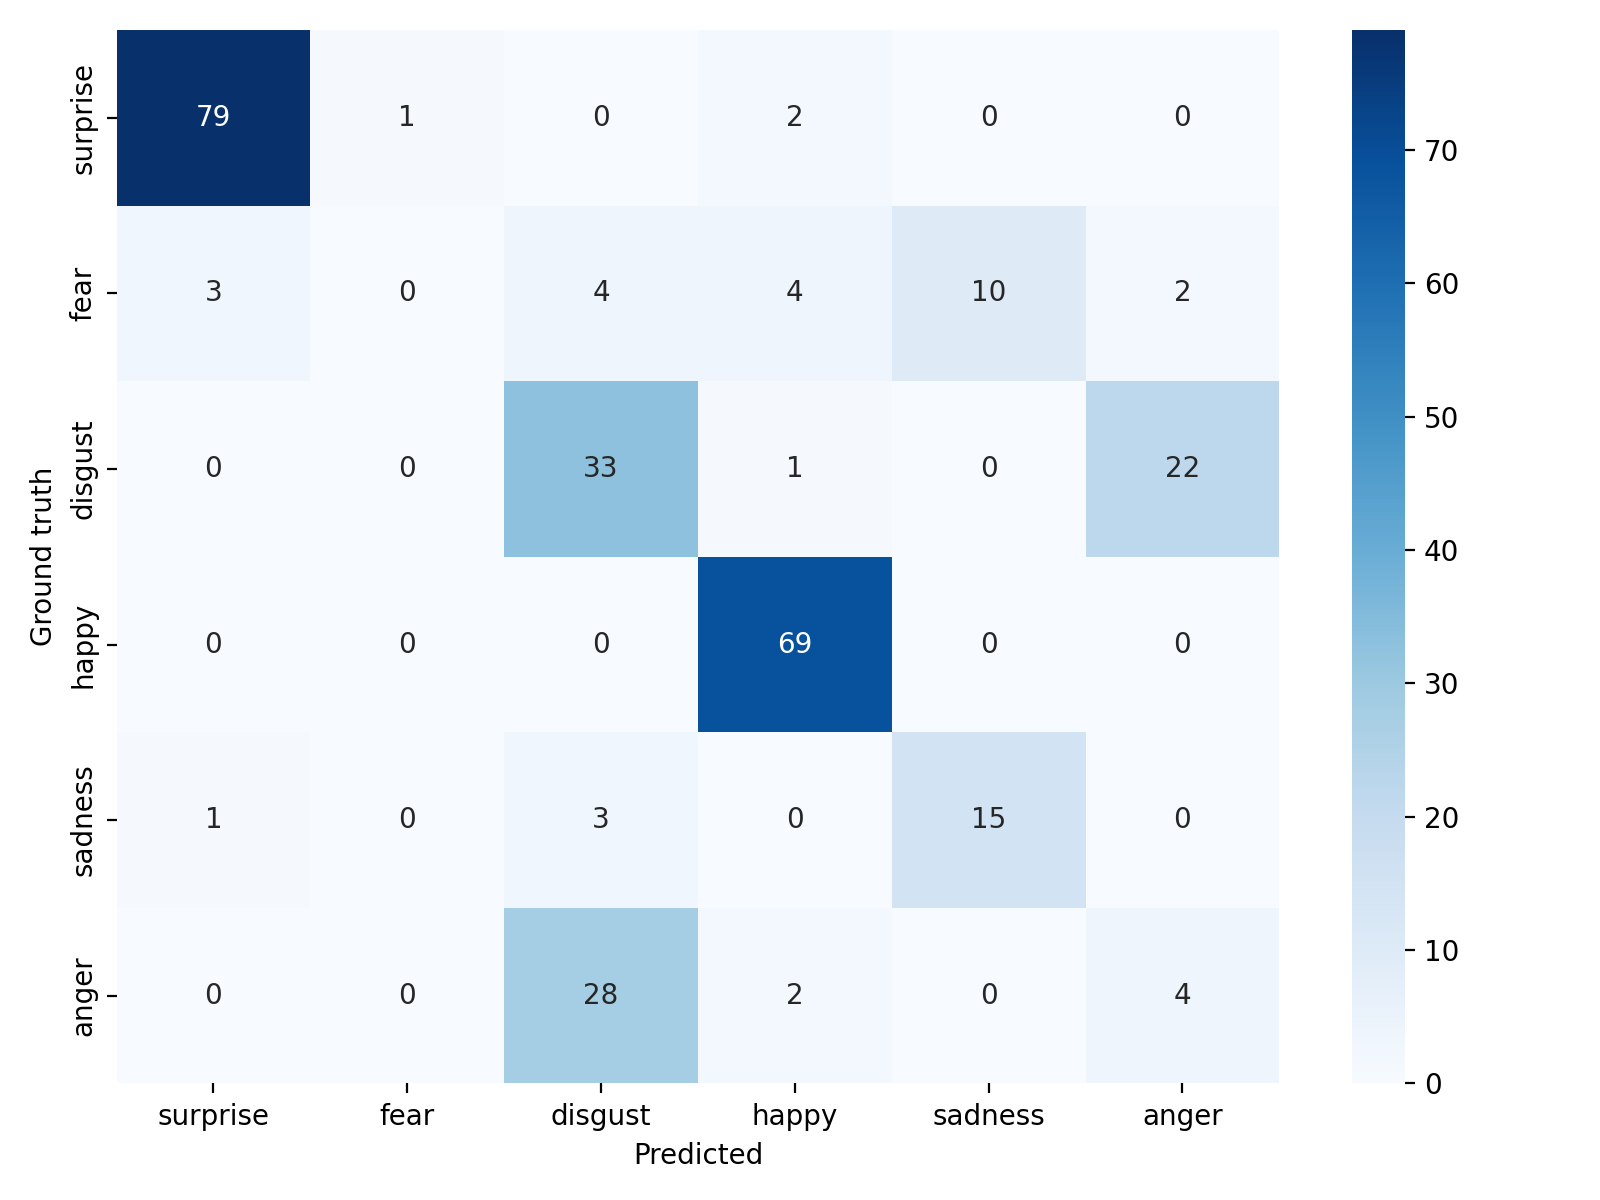
\includegraphics[width=\textwidth]{images/cm_ckplus48_peak.png}
        \caption*{(f) CK+48 6 lớp peak-only (309 mẫu)}
    \end{minipage}

    \caption{Ma trận nhầm lẫn của mô hình CAFE trên sáu tập đánh giá chéo miền (huấn luyện trên RAF-DB, không tinh chỉnh trên miền đích). Trục dọc là nhãn thực tế (Ground truth), trục ngang là nhãn dự đoán (Predicted).}
    \label{fig:cm_all}
\end{figure}


\subsection{Phân tích sai khác và thảo luận}
% Thảo luận các nguyên nhân có thể làm kết quả khác với bài báo, chẳng hạn khác biệt về bộ dữ liệu, cấu hình huấn luyện, phần cứng, số epoch, chiến lược tiền xử lý hoặc yếu tố ngẫu nhiên.

Sai khác giữa kết quả của nhóm và bài báo gốc đến từ nhiều nguyên nhân. Trước hết, mặc dù nhóm sử dụng cùng ý tưởng huấn luyện trên RAF-DB và đánh giá chéo miền, môi trường chạy lại không hoàn toàn trùng khớp với thiết lập gốc của tác giả. Các yếu tố như phiên bản thư viện, GPU, cách tải checkpoint CLIP, seed, batch size và chiến lược đọc dữ liệu đều có thể tạo sai khác nhỏ trong quá trình tối ưu.

Thứ hai, các bộ dữ liệu được lấy từ nguồn Kaggle có cấu trúc thư mục và quy ước nhãn không đồng nhất. FERPlus có thư mục \textit{contempt} bị loại bỏ; AffectNet cũng bỏ lớp \textit{Contempt}; SFEW2.0 sử dụng tập Val vì tập Test không có nhãn trong cấu trúc dữ liệu hiện có. Những điều chỉnh này cần thiết để ánh xạ về bảy lớp của CAFE, nhưng đồng thời làm giao thức đánh giá khác một phần so với bài báo. Riêng hai tập FERPlus và SFEW2.0, sự kết hợp của các yếu tố này dẫn đến chênh lệch lần lượt $-6.35\%$ và $-5.99\%$ so với kết quả bài báo gốc --- đây là những trường hợp tái hiện không đạt đầy đủ cần được ghi nhận rõ.

Thứ ba, CK+48 là một trường hợp mở rộng ngoài các tập chính trong bài báo. Ảnh CK+48 có độ phân giải 48 $\times$ 48, sau đó được phóng lên $224 \times 224$ để phù hợp với đầu vào của mô hình. Quá trình phóng đại này không tạo thêm chi tiết khuôn mặt mới, nên các đặc trưng vi mô của những cảm xúc khó như \textit{fear} hoặc \textit{anger} có thể bị mất hoặc không đủ rõ. Quan sát ma trận nhầm lẫn tại Hình~\ref{fig:cm_all}(e)-(f), toàn bộ 25 mẫu \textit{fear} bị phân tán sang các lớp khác (chủ yếu \textit{sadness} và \textit{happy}), xác nhận mô hình không có khả năng nhận diện \textit{fear} trong điều kiện ảnh phóng đại từ độ phân giải thấp.

Thứ tư, phân phối lớp giữa các bộ dữ liệu mất cân bằng rõ rệt. Minh chứng rõ nét nhất là ở bộ dữ liệu mở rộng CK+48 đã được nhóm phân tích trực quan qua biểu đồ phân phối mẫu tại Hình~\ref{fig:ckplus_distribution}. Sự mất cân bằng cực đoan này giải thích lý do vì sao ở chế độ 7 lớp, Overall Accuracy đạt mức rất cao ($82.48\%$), nhưng Mean Accuracy và Macro-F1 lại thấp hơn nhiều ($57.90\%$ và $53.73\%$), do mô hình nhận diện tốt lớp chiếm đa số (\textit{neutral}, \textit{happy}) nhưng đoán sai các lớp ít mẫu như \textit{fear} hay \textit{anger}. Khi chuyển sang chế độ 6 lớp peak-only, việc loại bỏ hoàn toàn lớp \textit{neutral} giúp phản ánh thực chất và công bằng hơn năng lực nhận dạng cảm xúc thực tế của mô hình.

Thứ năm, nhìn vào các ma trận nhầm lẫn trong Hình~\ref{fig:cm_all}, có thể rút ra hai pattern lỗi hệ thống của mô hình CAFE. \textbf{Pattern thứ nhất} là sự hút về trung tâm của \textit{happy} và \textit{neutral}: trên SFEW2.0, phần lớn mẫu \textit{surprise} (19/56), \textit{fear} (10/46) và \textit{disgust} (5/23) đều bị dự đoán nhầm sang \textit{sadness} hoặc \textit{neutral}, cho thấy mô hình bị thiên hướng về các lớp đông mẫu trong tập huấn luyện RAF-DB. \textbf{Pattern thứ hai} là sự nhầm lẫn giữa \textit{anger} và \textit{disgust}: trên CK+48, 28/45 mẫu \textit{anger} bị phân loại thành \textit{disgust} do hai biểu cảm này có nhiều điểm tương đồng về chuyển động cơ vùng miệng và lông mày.

Từ các kết quả trên, có thể nhận xét rằng CAFE giữ được năng lực tổng quát hóa tương đối tốt khi chuyển từ RAF-DB sang các bộ dữ liệu ngoài miền. Tuy nhiên, mô hình vẫn chưa giải quyết triệt để các lớp cảm xúc mơ hồ, các bộ dữ liệu có ảnh chất lượng thấp hoặc các trường hợp phân phối lớp lệch mạnh. Do đó, trong báo cáo này, Overall Accuracy được dùng để so sánh với bài báo gốc, còn Mean Accuracy và Macro-F1 được dùng để phân tích sâu hơn về tính cân bằng của mô hình.
\subsection{Mở rộng hoặc cải tiến}
% Nếu nhóm thực hiện phần điểm thưởng, trình bày rõ cải tiến hoặc mở rộng, ví dụ áp dụng mô hình trên bộ dữ liệu mới, thay đổi kiến trúc, bổ sung chiến lược tăng cường dữ liệu hoặc tối ưu tốc độ suy luận.


Ngoài việc chạy lại huấn luyện và đánh giá trên các bộ dữ liệu được đề cập trong bài báo, nhóm thực hiện thêm hai mở rộng. Mở rộng thứ nhất là xây dựng script đánh giá CK+48. Đây là bộ dữ liệu có đặc điểm khác biệt so với RAF-DB và các tập dữ liệu in-the-wild vì ảnh có độ phân giải thấp, nhiều mẫu được thu trong điều kiện phòng thí nghiệm và có thể bao gồm cả mẫu trung tính.Việc đánh giá trên hai chế độ CK+48, gồm 6 lớp peak-only và 7 lớp có neutral, giúp quan sát rõ ảnh hưởng của cách chọn mẫu và ánh xạ nhãn đến kết quả.

Mở rộng thứ hai là chuẩn hóa pipeline đánh giá chéo miền cho nhiều bộ dữ liệu thư mục. Script \texttt{evaluate\_cross\_dataset.py} tự động nhận diện split, bỏ lớp \textit{contempt} khi cần, ánh xạ tên lớp về thứ tự nhãn của CAFE và lưu đồng nhất các file \texttt{predictions.csv}, \texttt{metrics.json} và \\ \texttt{confusion\_matrix.png}. Nhờ đó, quá trình so sánh giữa FERPlus, AffectNet, SFEW2.0 và \\ MMAFEDB trở nên nhất quán hơn và dễ kiểm tra lại.

Trong các hướng cải tiến tiếp theo, nhóm đề xuất bổ sung cơ chế cân bằng lớp khi đánh giá và huấn luyện, chẳng hạn weighted loss hoặc balanced sampler, để giảm thiên lệch về các lớp phổ biến như \textit{happy} và \textit{neutral}. Ngoài ra, có thể kết hợp thêm dữ liệu khuôn mặt độ phân giải thấp hoặc chiến lược tăng cường dữ liệu mô phỏng nhiễu, mờ, lệch sáng để cải thiện hiệu quả trên CK+48 và SFEW2.0. Cuối cùng, nếu mở rộng sang video, việc bổ sung mô-đun thời gian như GRU hoặc Transformer temporal adapter có thể giúp mô hình phân biệt tốt hơn các cảm xúc dễ nhầm lẫn trên ảnh tĩnh.


\subsection{Demo minh họa}
Dự án cung cấp hai ứng dụng demo webcam theo thời gian thực cho nhận dạng biểu cảm khuôn mặt. Demo thứ nhất  sử dụng mô hình CAFE đã được huấn luyện kết hợp CLIP ViT-B/32 và ResNet-18 để nhận dạng bảy loại biểu cảm (surprise, fear, disgust, happy, sadness, anger, neutral). Demo thứ hai không cần checkpoint mà sử dụng CLIP pure zero-shot với multiple text prompts. Cả hai demo đều thực hiện quy trình: phát hiện khuôn mặt từ webcam, cắt vùng khuôn mặt, tiền xử lý ảnh, dự đoán biểu cảm, và hiển thị kết quả trực tiếp lên frame video.

\begin{itemize}
    \item \textbf{Đầu vào:}  webcam.
    \item \textbf{Đầu ra:} Nhãn dự đoán, quyết định xác minh.
    \item \textbf{Thư viện/công cụ:} PyTorch, OpenCV, pillow, scikit-learn, ftfy, \dots
    \item \textbf{Kịch bản chạy:} Chạy source code demo và thực hiện thay đổi các biểu cảm trên khuôn mặt.
    \item \textbf{Link video:} \href{https://drive.google.com/drive/folders/1BC7GI7or8lLDn4QfEYbvI_TSbq7936Fp}{Video demo CLIP + CAFE}.
    \item \textbf{source code demo:} \href{https://github.com/DinhLiu/Generalizable-FER}{Source code demo}
\end{itemize}